\chapter{Organisation du travail}

\section{Répartition des tâches}

Comme le projet peut être découpé en plusieurs blocs qui peuvent être
développés de manière presque indépendante, nous nous sommes répartis
par équipe sur chaque bloc. Certains blocs nécessitent
cependant une base provenant d’autres blocs pour faire des tests.
Par exemple, la partie IHM aura besoin d’une base de données pour
vérifier que la recherche d’imagettes dans celle-ci se déroule bien.
Nous allons donc commencer par développer des prototypes simplifiés
pour que tout le monde puisse améliorer sa partie. De plus, certains 
blocs ne représentent pas la même quantité de travail, certaines 
personnes sont donc réparties sur plusieurs blocs.

\paragraph{}
Voici la répartition que nous avons effectuée sur les différents blocs :

\begin{center}

\begin{tabular}{ | l | l | }
	\hline
	\multicolumn{2}{ | c | }{ \textbf{Bloc 1 : Préparation des données} } \\
	\hline
	\textbf{Spécification} & \textbf{Description} \\
	\hline
	PR\_FO\_1 & Traiter le format PiFF en interne dans le logiciel \\
	\hline
	PR\_FO\_2 & Fournir un convertisseur du format GEDI vers PiFF \\
	\hline
	PR\_TR\_1 & Intégrer une fonction de détection de lignes au logiciel \\
	\hline
	PR\_TR\_2 & Permettre un découpage des images en lignes \\
	\hline
	PR\_TR\_3 & Localiser les paragraphes \\
	\hline
	PR\_TR\_4 & Permettre un découpage des images en paragraphes \\
	\hline
	PR\_RE\_1 & Associer les images à leur transcription \\
	\hline
	PR\_RE\_2 & Associer la vérité terrain à une transcription \\
	\hline
	PR\_RE\_3 & Permettre de générer une vérité terrain si besoin, grâce à un reconnaisseur \\
	\hline
\end{tabular}

\paragraph{}
\begin{tabular}{ | l | l | }
	\hline
	\multicolumn{2}{ | c | }{ \textbf{Bloc 2 : Stockage des données} } \\
	\hline
	\textbf{Spécification} & \textbf{Description} \\
	\hline
	STO\_VER & Stocker des imagettes associées à une vérité terrain \\
	\hline
	STO\_USR & Stocker des imagettes associées à une transcription générée par l’utilisateur \\
	\hline
	STO\_REC & Stocker des imagettes associées à une transcription générée par un reconnaisseur  \\
	\hline
	STO\_SEL & Fournir des méthodes pour accéder aux données stockées  \\
	\hline
	STO\_UPD & Fournir des méthodes pour modifier les données stockées \\
	\hline
	STO\_INS & Fournir des méthodes pour pouvoir insérer des données à stocker \\
	\hline
	STO\_DEL & Fournir des méthodes pour pouvoir supprimer des données stockées \\
	\hline
\end{tabular}

\paragraph{}
\begin{tabular}{ | l | l | }
	\hline
	\multicolumn{2}{ | c | }{ \textbf{Bloc 3 : Interface avec le reconnaisseur} } \\
	\hline
	\textbf{Spécification} & \textbf{Description} \\
	\hline
	IR\_CV & Convertir les données au format d’entrée du reconnaisseur \\
	\hline
	IR\_AP & Fournir les données au reconnaisseur \\
	\hline
	IR\_EV & Pouvoir lancer une évaluation du reconnaisseur  \\
	\hline
	IR\_TR & Pouvoir lancer une transcription d’un document par le reconnaisseur   \\
	\hline
\end{tabular}

\newpage

\begin{tabular}{ | l | p{0.8\linewidth} | }
	\hline
	\multicolumn{2}{ | c | }{ \textbf{Bloc 4 : Interface avec l’utilisateur} } \\
	\hline
	\textbf{Spécification} & \textbf{Description} \\
	\hline
	PEA\_GEN\_1 & Valider un ensemble d'annotations \\
	\hline
	PEA\_GEN\_2 & Éditer manuellement les transcriptions \\
	\hline
	PEA\_GEN\_3 & Corriger les annotations proposées par un reconnaisseur externe à l'application \\
	\hline
	PEA\_GEN\_4 & Envoyer les modifications à la base de données lorsque la vérité-terrain d’une imagette est modifiée \\
	\hline
	PEA\_GEN\_5 & Ignorer un couple imagette-transcription s’il n’est pas pertinent \\
	\hline
	PEA\_GEN\_6 & Regrouper les documents en projets \\
	\hline
	PEA\_GEN\_7 & Sélectionner d’abord le projet puis le document sur lequel l’utilisateur veut travailler à l’ouverture de l’application \\
	\hline
	PEA\_GEN\_8 & Créer un nouveau projet \\
	\hline
	PEA\_GEN\_9 & Basculer vers la page de découpe des zones \\
	\hline
	PEA\_GEN\_10 & Basculer vers la page d’édition des annotations \\
	\hline
	PEA\_GEN\_11 & Basculer vers la page de validation des transcriptions \\
	\hline
	PDEC\_OD\_1 & Créer une nouvelle zone à l’aide d’un rectangle (outil "nouvelle sélection") \\
	\hline
	PDEC\_OD\_2 & Pouvoir modifier la position des sommets des rectangles \\
	\hline
	PDEC\_OD\_3 & Rajouter des sommets à la zone \\
	\hline
	PDEC\_OD\_4 & Changer le type de la zone avec un menu déroulant \\
	\hline
	PDEC\_OD\_5 & Déplace la zone sélectionnée sur le document (outil “déplacer”) \\
	\hline
	PDEC\_OD\_6 & Zoomer et dézoomer sur le document (outils “zoom +” et “zoom -”) \\
	\hline
	PDEC\_OD\_7 & Annuler la dernière action (outil “annuler”) \\
	\hline
	PDEC\_OD\_8 & Refaire l’action annulée précédemment (outil “refaire”) \\
	\hline
	PDEC\_OD\_9 & Supprime toutes les zones de la page pour retourner au document vierge (outil “réinitialiser”) \\
	\hline
	PDEC\_OD\_10 & Applique un détecteur de lignes sur la zone sélectionnée (outil “appliquer la détection de lignes sur la zone”) \\
	\hline
	PDEC\_OD\_11 & Continuer la découpe du document sur la page suivante \\
	\hline
	PDEC\_OD\_12 & Passer à l’édition des annotations sur la page qu’il vient de découper \\
	\hline
	PDEC\_OD\_13 & Exporter la page découpée au format PiFF afin de soumettre les données à un reconnaisseur externe à l’application \\
	\hline
	PDEC\_OD\_14 & Posséder un bouton de retour au menu principal \\
	\hline
	PDEC\_OD\_15 & Permettre à l’utilisateur de se déplacer sur le manuscrit à l’aide d’un scroll horizontal et vertical \\
	\hline
	PEMA\_1 & Placer le curseur sur la première imagette ne possédant pas de transcription \\
	\hline
	PEMA\_2 & Positionner le curseur sur l’annotation suivante en appuyant sur Entrée \\
	\hline
	PEMA\_3 & Proposer un raccourci clavier permettant de basculer vers la prochaine imagette sans vérité-terrain \\
	\hline
	PEMA\_4 & Posséder un bouton intitulé “modifier les zones du manuscrit” \\
	\hline
	PEMA\_5 & Afficher la liste des imagettes du document découpé \\
	\hline
	PEMA\_6 & Ignorer un couple imagette-transcription s’il n’est pas pertinent \\
	\hline
	PEMA\_7 & Basculer vers la page de validation des transcriptions \\
	\hline
	PCORIA\_1 & Valider les transcriptions zone par zone et passer à la zone suivante avec un simple appui sur Entrée \\
	\hline
	PCORIA\_2 & Pouvoir modifier une annotation fausse en cliquant dessus pour y positionner son curseur et en effectuant ses modifications manuellement \\
	\hline
	PCORIA\_3 & La zone de visualisation des imagettes se présente de la même manière que sur la page d’édition manuelle des transcriptions \\
	\hline
	PCORIA\_4 & Posséder également la fonctionnalité de mise à l’écart d’un couple imagette-transcription \\
	\hline
	PCORIA\_5 & Basculer vers la page de validation des transcriptions \\
	\hline
\end{tabular}

\begin{tabular}{ | l | p{0.8\linewidth} | }
	\hline
	\textbf{Spécification} & \textbf{Description} \\
	\hline
	PVAL\_1 & Accéder à la page de validation depuis le menu principal \\
	\hline
	PVAL\_2 & Accéder à cette page de validation depuis les pages d’édition manuelle des annotations et de correction des transcriptions proposées par le reconnaisseur \\
	\hline
	PVAL\_3 & Valider les transcriptions zone par zone et passer à la zone suivante avec un simple appui sur Entrée \\
	\hline
	PVAL\_4 & Pouvoir modifier une annotation fausse en cliquant dessus pour y positionner son curseur et en effectuant ses modifications manuellement \\
	\hline
	PVAL\_5 & Indique si les transcriptions ont été fournies manuellement par un humain ou si elles proviennent d’un reconnaisseur \\
	\hline
	PVAL\_6 & Faire figurer une fenêtre montrant la page entière découpée en zones avec la zone courante dans une couleur différente \\
	\hline
	PVAL\_7 & Valider le travail pour de bon et fermer le document à l’aide d’un bouton prévu à cet effet \\
	\hline
\end{tabular}

\paragraph{}
\begin{tabular}{ | l | l | }
	\hline
	\multicolumn{2}{ | c | }{ \textbf{Bloc 5 : Lien entre les blocs précédents} } \\
	\hline
	\textbf{Spécification} & \textbf{Description} \\
	\hline
	LINK\_PR\_STO & Envoyer les données en entrée vers le système de stockage \\
	\hline
	LINK\_STO\_IHM & Extraire les données pour les fournir à l’IHM \\
	\hline
	LINK\_STO\_IR & Extraire les données pour les fournir au système de reconnaissance \\
	\hline
	LINK\_IHM\_STO & Envoyer les demandes de l’IHM au système de stockage \\
	\hline
	LINK\_IHM\_IR & Envoyer les résultats du reconnaisseur vers le système de stockage \\
	\hline
	LINK\_COH & Fournir un logiciel composés de blocs communiquant entre eux de manière fonctionnelle et cohérente \\
	\hline
\end{tabular}

\end{center}

\paragraph{}
\begin{tabular}{ | l | l | }
	\hline
	\multicolumn{2}{ | c | }{ \textbf{Bloc 6 : Général} } \\
	\hline
	\textbf{Spécification} & \textbf{Description} \\
	\hline
	GEN\_ERGO & Ergonomie de l‘application \\
	\hline
	GEN\_ERGO & Concevoir un logiciel évolutif \\
	\hline
	GEN\_ERGO & Fournir un logiciel open source \\
	\hline
\end{tabular}

\end{center}

\paragraph{}

Ainsi nous nous répartissons le travail selon ces blocs : Enzo CRANCE et
Valentin FOUCHER s’occupent du bloc 1, Kévin DESPOULAINS, Corentin GUILLOUX et Valentin FOUCHER
du bloc 2, Gaël GENDRON et Timothée NEITTHOFFER du bloc 3, Laure DU MESNILDOT et Charlotte
RICHARD du bloc 4, Gaël GENDRON et Timothée NEITTHOFFER du bloc 5. 

\paragraph{}
Cette répartition des tâches permet à chaque équipe de spécifier plus en détail
sa partie, et donc de pouvoir estimer plus précisément le temps que prendra le
développement. Nous espérons donc avoir un rapport de planification précis qui
nous permettra d’anticiper d’éventuelles réorganisations d’équipes en fonction
des différentes charges de travail.

\paragraph{}
Nous fonctionnerons de manière itérative pour s’assurer régulièrement du fonctionnement
 des blocs seuls et entre eux. Pour le moment, deux itérations ont été planifiées mais
 nous envisageons de redécouper le travail en plusieurs nouvelles itérations. Cette
 organisation, décrite dans la partie suivante, sera abordée plus en détail dans 
le rapport de planification.

\section{Organisation temporelle}

Certains membres du groupe partent en mobilité en janvier (Kévin DESPOULAINS,
Corentin GUILLOUX, et Gaël GENDRON). Notre premier objectif est donc de
concevoir la base et la documentation de chaque partie avant leur départ.
Nous allons donc anticiper la phase de développement en la débutant dès à
présent. Le diagramme de Gantt précédemment établi se trouve donc modifié de
cette manière :

\newpage

\begin{mdframed}[frametitle={Figure 17 : Estimation de la planification des tâches}, innerbottommargin=10]
\begin{center}
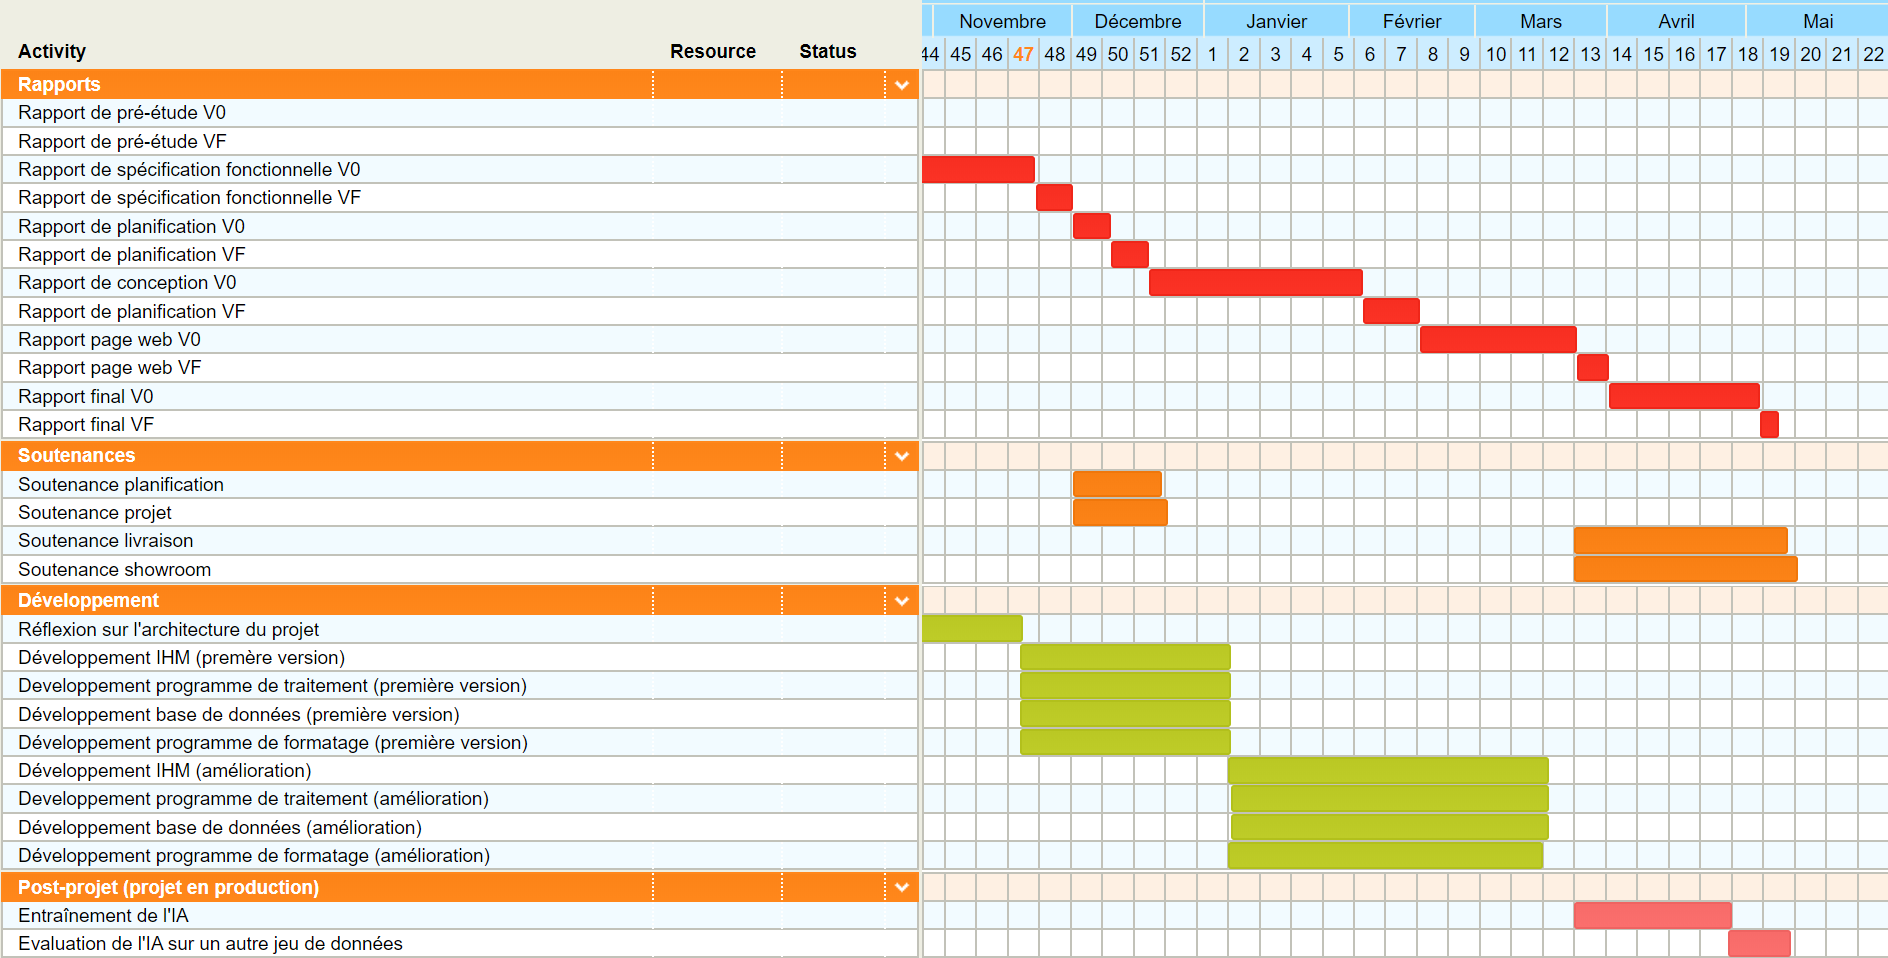
\includegraphics[scale=0.5]{gantt.png}
\end{center}
\end{mdframed}

\paragraph{}
\underline{Légende}

\paragraph{}
\textcolor{red}{En rouge : } rédaction des différents livrables. Nous avons estimé que le début de rédaction d’un livrable doit se faire dès le rendu du livrable précédent.

\paragraph{}
\textcolor{orange}{En orange : } soutenances. Les dates de début de préparation sont pour l’instant difficiles à définir, la taille des blocs est donc provisoire.

\paragraph{}
\textcolor{green}{En vert : } développement. Comme on peut le voir, il y a plusieures parties du développement qui se font en parallèle. Les durées de chaques parties sont prévisionnelles mais sont susceptibles d’être grandement modifiées.

\paragraph{}
\textcolor{pink}{En rose : } exécution du projet en mode production. Ce seront les tests du reconnaisseur.
